\section{User Testing} \label{sec:s4_test}
%%% Intro paragraph

The previous section presents how the local crowd factors are visualised. Although the visualisation displays a lot of information about a crowd, it does not necessarily mean that the information is useful in the domain of crowd safety. This section describes how we test the usefulness of the visualised information and the application in general.

\subsection{Test Method}
Anders Nord, who is part of Alarm HS, kindly agreed to participate in this user test. The user test was performed, as the other meetings, over Skype. Anders was presented with the application which was configured to display the following predefined crowd scenarios. We will in this test not consider the pressure overlay, because we estimated that it would be difficult to explain the concept in detail.  

The first scenario was a very simple \enquote{tutorial}. Its purpose is to give Anders an intuition of how the density, velocity and turbulence overlays behave and the information they can provide. \Cref{fig:tutorial_screens} provides a visual illustration of this. The top two groups is showing how density, velocity and turbulence overlays work.

\begin{figure}[htbp]
\begin{subfigure}[t]{.49\linewidth}
    \centering
    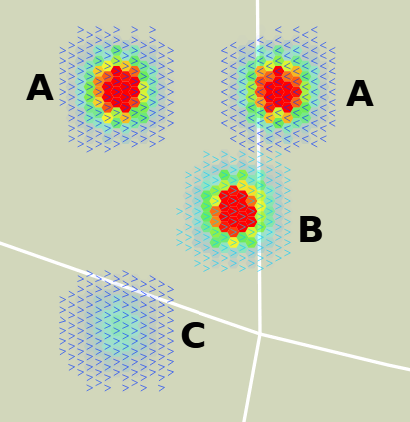
\includegraphics[width=\linewidth]{velocity_density_tutorial.png}
    \caption{Velocity and density - The top three groups are all more dense than the bottom group. The third group from the top moves at a faster rate than the rest.}
\end{subfigure}
\enspace
\begin{subfigure}[t]{.49\linewidth}
    \centering
    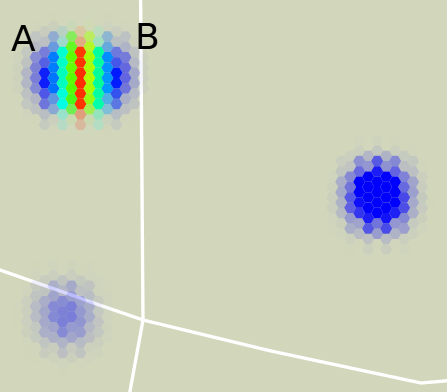
\includegraphics[width=\linewidth]{turbulence_tutorial.png}
    \caption{Turbulence - The top two groups are \enquote{crashing} which shows up as high turbulence.}
\end{subfigure}
\caption{Screenshots of the tutorial scenario}
\label{fig:tutorial_screens}
\end{figure}

After the tutorial scenario, we switched to a more detailed data set. The data set resembles a normal day on SmukFest, and is artificially created by us. The data contains a variety of interesting situations. A large, dense crowd is standing in front of a stage. South of the stage, people are moving in an oddly shaped infinity sign. This means that there is a crossroad, where groups of people are meeting. In the top left corner of the area, people are moving in opposite directions close to each other. \Cref{fig:test_data_screens} shows this visualised. 

\begin{figure}[htbp]
\begin{subfigure}[t]{.49\linewidth}
    \centering
    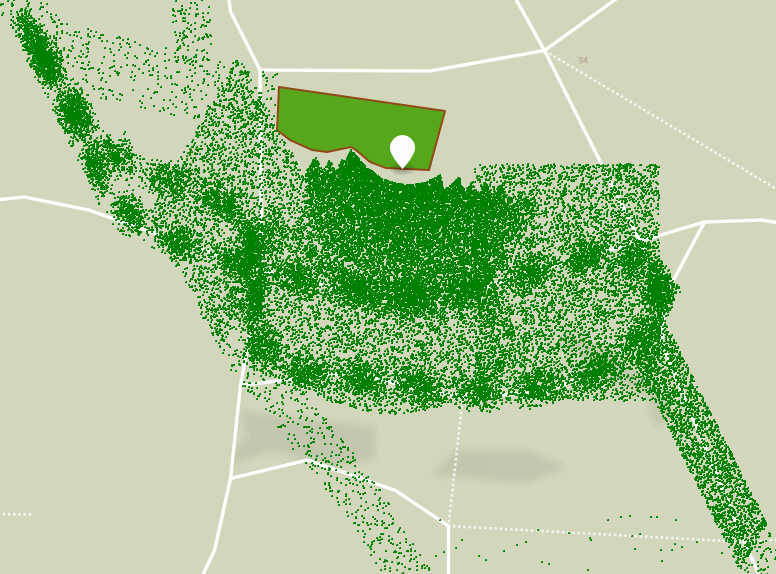
\includegraphics[width=\linewidth]{people_test_data.png}
    \caption{Distribution of people - Each green dot is a person.}
\end{subfigure}
\enspace
\begin{subfigure}[t]{.49\linewidth}
    \centering
    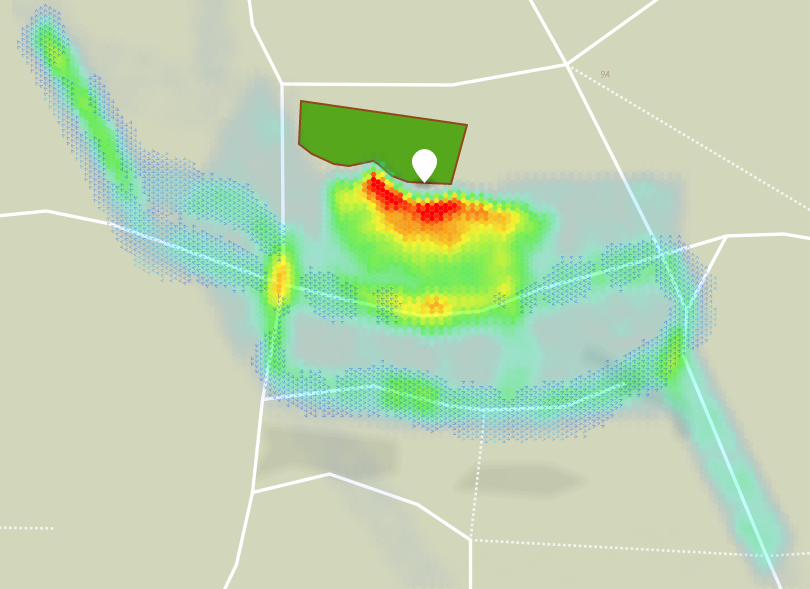
\includegraphics[width=\linewidth]{velocity_density_test_data.png}
    \caption{Velocity and density - The density is very high at the front of the stage and also at a few positions where multiple groups of people meet. Velocity can be seen at the oddly shaped infinity sign south of the stage.}
\end{subfigure}
\enspace
\begin{subfigure}[t]{.49\linewidth}
    \centering
    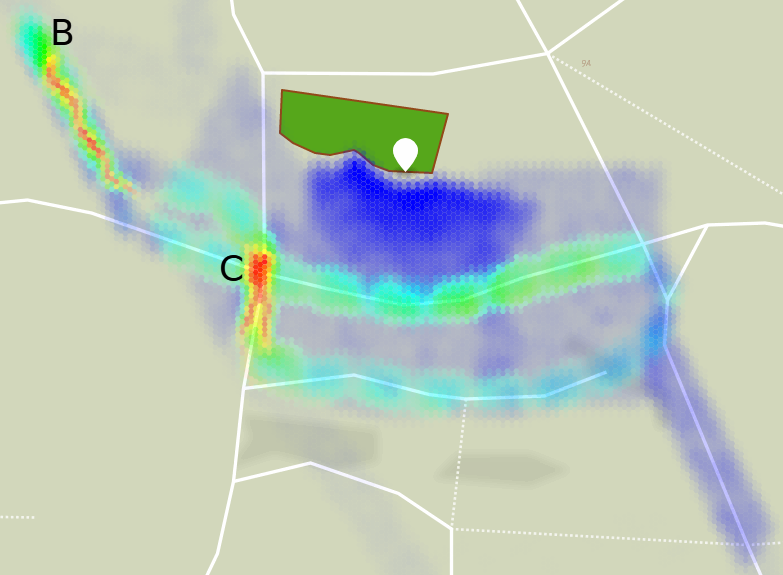
\includegraphics[width=\linewidth]{turbulence_test_data.png}
    \caption{Turbulence - The turbulence is high at two positions; at the crossroads of the oddly shaped infinity sign and at the very top left corner. Even though the density was very high at the front of the stage, which could be dangerous, it turns out that the turbulence is low, meaning that people are standing close to each other. This would indicate that the high density area in front of the stage is a small threat.}
\end{subfigure}
\caption{Screenshots of the test data scenario}
\label{fig:test_data_screens}
\end{figure}

In order to measure the performance of the system, we asked Anders to analyse this test data scenario. The idea being that if the system could visualise the data set in a good way, Anders would be able to find the interesting situations hidden in the data set.

%%% Testing results, high abstraction level
\subsection{Test Results}
Anders immediately noticed, using the density overlay, that the density was high in front of the stage, and at the crossroads where people meet. 

Switching to the velocity overlay, he did not immediately notice the arrows, as they were small. When we hinted that there were arrows, he was able to find the cycle of moving people in the oddly shaped infinite sign. Having both the velocity and density overlays enabled at the same time, Anders understood why the density was high at the crossroads; Many groups were heading to the crossroad.

The meaning of the turbulence overlay was not completely clear to Anders as he turned it on, but he quickly noticed that there was no turbulence at the area in front of the stage. His hypothesis was that the crowd was standing still at the area, which we could confirm. He also noticed the high turbulence at the crossroad and at the top left corner.

\subsection{Summary}
Overall, Anders was able to find all the interesting situations we had put in the test data, meaning that the visualisations of the system were good. He expressed that he was not completely confident in his knowledge about what each overlay represents. He suggested that a user of the system receives some sort of training on the system.







